\addchap{Grußwort}

\begin{wrapfigure}{l}{0.32\textwidth}
  \vspace{-15pt}
  \begin{centering}
    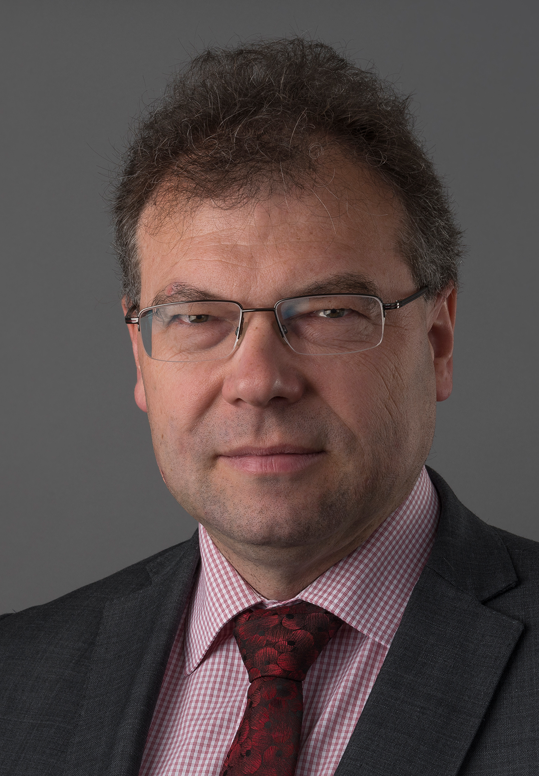
\includegraphics[width=0.3\textwidth]{img/uweassmann.png}
  \end{centering}
  \vspace{-20pt}
\end{wrapfigure}

Liebe Studentinnen und Studenten,

herzlichen Glückwunsch zum Beginn eines der spannendsten Studien, die es gibt, an einer der attraktivsten Informatikfakultäten Deutschlands und Europas!

Als Dekan ist es mir eine Freude, Sie herzlich an unserer Fakultät Informatik begrüßen zu dürfen. Mit 28 Professoren, 4 Honorarprofessoren, mehr als 300 Mitarbeitern und mehr als 1600 Studenten gehört die Fakultät zu den größten Informatikfakultäten Deutschlands mit einem der breitesten Spektren an Studieninhalten. Um unser modernes Gebäude werden wir von vielen anderen Fakultäten beneidet, auch wenn es manchmal mit einem Augenzwinkern als "Grünes Gewölbe" bezeichnet wird. Ich kann Ihnen aus eigener Erfahrung versichern: man gewöhnt sich an die Farbe. Das Gebäude bietet nicht nur Platz für die Mitarbeiter der Fakultät, sondern verfügt auch über einen Vorlesungssaal, diverse Seminarräume und hochwertig ausgestattete Rechner-Pools. Im Foyer liefert das Studentencafè ascii den für einen Wissenschaftsbetrieb äußerst wichtigen Koffeinnachschub. Was unser Kunstwerk im Foyer bedeutet, dürfen Sie gerne raten. Hinter unserem Gebäude lädt das "Nöthnitzer Meer" zum Lernen, Chillen und Sonnen ein. Bald wird auch unser Sportzentrum, gleich links von der Fakultät, wieder geöffnet sein.

Die Informatik durchdringt unsere Gesellschaft wie keine andere Wissenschaft und beschleunigt den wissenschaftlichen Fortschritt anderer Disziplinen enorm. Marc Andreesen, der Erfinder des ersten kommerziellen Web-Browsers "Netscape", prägte in 2011 den Slogan "Software is eating the world", was sagen will, dass die Digitalisierung alle Industrien und alle Lebensbereiche verändert. Software läuft nicht nur in Computern, sondern auch in Autos, Flugzeugen, Wasch- und Kaffeemaschinen. Computerprogramme erledigen heute Aufgaben, die noch vor 20 Jahren Biologiestudenten einen Doktortitel eingebracht hätten. Teilweise ist der Einfluss von Software sogar so tief, dass er der Gesellschaft gar nicht mehr bewusst ist: Wer denkt heute schon darüber nach, dass sein Handy aus einem Berg voller Software besteht? Die Digitalisierung führt auch dazu, dass Firmen händeringend nach Informatikern suchen. Unsere Fakultät kann derzeit mit ihren Absolventen nicht einmal den Fachkräftebedarf der Software-Industrie im Raum Dresden decken, denn sie wächst jedes Jahr um ca. 5 - 7\% und benötigt dazu ca. 600 neue Informatiker. Nach dem erfolgreichen Abschluss Ihres Studiums werden Ihnen daher viele Türen offenstehen. Also zunächst einmal herzlichen Glückwunsch zu diesen guten Aussichten!

Ich hoffe jedoch, dass Sie sich nicht nur wegen der guten Job-Aussichten für das Studium der Informatik entschieden haben, sondern auch wegen Ihres Interesses am Fach und Ihrer Freude am Lernen. Wir freuen uns auf jeden Fall darauf, Sie auf Ihrem Weg der Bildung und des Lernens zu begleiten.

Für Sie, liebe Studentinnen und Studenten, beginnt mit dem Studium ein neuer, faszinierender Lebensabschnitt, der mehr Freiheiten bietet als die Schule vorher und das Berufsleben danach. Diese Freiheiten sollten Sie nutzen, um sich in freier Selbstbestimmung zu bilden, Ihr Studium selbst zu planen, Ihre Lerninhalte selbst zu vertiefen und sich selbst Ihre Lern-Arbeit einzuteilen. Das macht Spaß - es bringt aber auch zwei Probleme mit sich: Erstens muss man das systematische Erarbeiten von großen Mengen an Lernstoff trainieren, und zweitens benötigt man für ein erfolgreiches Studium mehr Disziplin, als man von der Schule gewohnt ist. Also, einige Tipps: Gehen Sie bitte regelmäßig in die Vorlesungen, denn der Professor fasst dort für Sie die wichtigsten Inhalte des Fachgebiets zusammen, so dass Sie schnell Wichtiges von Unwichtigem unterscheiden können. Bereiten Sie bitte diese Kerninhalte Ihres Faches regelmäßig nach, denn dann verankern sie sich schneller in Ihrem Kopf - nichts ist schlimmer als eine Woche Bulimielernen vor der Prüfung. Schließlich: Erarbeiten Sie sich die Lösungen zu den Übungsaufgaben selbstständig, denn das selbstständige Lösen von Aufgaben führt Sie schnell zu einer höheren Stufe des Lernens und der damit verbundenen Leistungsfähigkeit (Bloomsche Lernzielhierarchie, siehe Wikipedia). Das erfolgreiche Herunterladen der Vorlesungsfolien oder des Skripts zur Vorlesung trägt nur dann zum Bestehen der Prüfung bei, wenn Sie sich auch intensiv mit den Inhalten auseinander setzen :-) Versuchen Sie, alle Begriffe zu verstehen und zusätzlich in der Lage zu sein, sie aktiv erklären zu können. Bitte versuchen Sie nicht, das Studium als Einzelkämpfer zu bewältigen, sondern nutzen Sie die Tatsache, dass Sie an einer großen Fakultät zusammen mit vielen Kommilitonen studieren, mit denen Sie Vorlesungsinhalte diskutieren und schwierige Themen gemeinsam erarbeiten können. Laden Sie sich gegenseitig zum Kaffee ins ASCII ein und erklären Sie sich dabei, was in der letzten Vorlesung behandelt worden ist. Das verbessert nicht nur den Studienerfolg, sondern macht auch viel mehr Spaß. (Das habe auch ich in meinem Studium so erlebt.) Und wenn Sie trotzdem im Studium auf Probleme stoßen, stehen Ihnen viele Anlaufstellen zur Verfügung: Studienfachberater, Mitglieder des Fachschaftsrates, Übungsgruppenleiter und selbstverständlich auch alle Professoren, die für Sie Sprechstunden anbieten, die Sie nutzen sollten, insbesondere zu einem Check vor Prüfungen.

Wenn ich an meinen eigenen Studienbeginn in 1982 in Karlsruhe zurückdenke, fällt mir zunächst ein, dass ich aus zeitlichen Gründen nicht an der damaligen ESE teilnehmen konnte. Das hat mich in den ersten Semestern sehr beeinträchtigt, denn ich fand mich außerhalb der Lerngruppen wieder, die sich in der ESE gebildet hatten, und lernte daher nur Schritt für Schritt die nötigen Lernpartner kennen. Daher bitte ich Sie: Sprechen Sie diejenigen, die noch keine Lerngruppe gefunden haben, an und laden Sie sie in Ihre Teams ein, denn es soll keiner auf dem Weg liegenbleiben. (Sie ahnen schon, warum wir das ascii eingerichtet haben...)

Das Humboldtsche Bildungsideal der Einheit von Forschung und Lehre besagt, dass ein Mensch sich bildet, indem er seine Welt erforscht. Daher legen die Universitäten in Deutschland großen Wert auf die Ausbildung in wissenschaftlichen Fertigkeiten und modernen Forschungsergebnissen. Lehre soll niemals nur Standardstoff vermitteln, sondern neue Erkenntnisse über die Welt und die Technologie.

Auch an der Fakultät Informatik der TU Dresden spielt das Humboldtsche Prinzip eine wichtige Rolle. Die Professoren und wissenschaftlichen Mitarbeiter der Fakultät beschäftigen sich in einer Vielzahl von Forschungsprojekten intensiv mit verschiedensten Grundlagen- und Anwendungsthemen. Seit dem 15. Juni 2012 ist die TU Dresden in den Kreis der "Exzellenzuniversitäten" aufgestiegen. Die Fakultät Informatik ist am Exzellenzcluster "Center for Advancing Electronics Dresden" beteiligt, der die Entwicklung neuer Technologien für das Computing der Zukunft zum Ziel hat, die die Begrenzungen heutiger CMOS-Technologie überwinden. Im Cluster forschen die Informatiker an Techniken, die sichere Berechnungen auch mit fehleranfälliger Hardware ermöglichen ("Resilienz"), sowie an Techniken zur Handhabung von Systemen mit sehr vielen und heterogenen Chips. Im Rahmen des Exzellenzclusters wurden an der Fakultät Informatik drei neue Professuren für Prozessordesign, Compilerbau und Wissensbasierte Systeme geschaffen, die das Vorlesungsangebot erweitern. Daneben hat die Fakultät zwei Doktorandenprogramme, sogenannte Graduiertenkollegs, in den Bereichen Theoretische Informatik und Software Engineering eingeworben. Sie ist damit eine der drei Informatikfakultäten Deutschlands, die mehrere solcher Programme anbieten können. Aber auch andere Drittmittelprojekte sowie vom Land finanzierte Stellen bieten Ihnen die Möglichkeit, im Anschluss an Ihr Studium an der TU Dresden zu promovieren.

Der olle Humboldt würde also sagen, dass die Forschungsaktivitäten der Fakultät nicht in Konkurrenz zu ihrer universitären Lehre stehen, sondern sie bedingen und "enablen" in vielerlei Hinsicht. Zum Beispiel ermöglichen es die Forschungsprojekte Ihnen, im Rahmen von Projekt-

und Abschlussarbeiten an der Lösung aktueller Forschungsfragen mitzuarbeiten, oder als bezahlte studentische Hilfskraft die ersten praktischen Erfahrungen mit der Softwareentwicklung zu sammeln. Unsere Projektpartner in der Industrie und anderen akademischen Einrichtungen bieten Ihnen interessante Industriepraktika und Auslandsaufenthalte, sowohl in Deutschland und Europa, als auch darüber hinaus. Und Sie erfahren in den Vorlesungen der späteren Jahre die neuesten Forschungsergebnisse oft aus erster Hand, und zwar von den Leuten, die sie entdeckt haben. Warum also nicht mit ihnen in eine Zusammenarbeit einsteigen? Wir freuen uns darauf.

Der größte Tag des Jahres ist für die Fakultät ihr "OUTPUT-DD"-Tag, der im nächsten Jahr am 15. Juni stattfindet. An diesem Tag wird in unserem Hause alles ausgestellt, was wir geforscht, entwickelt und gebaut haben: neue Ideen, neue Spiele, neue Filme, neue Informationssysteme, neue Roboterprogramme, neue Startups, etc. pp. Bitte heute schon vormerken und andere dazu einladen!

Am Ende meines Grußwortes möchte ich mich ganz herzlich beim Fachschaftsrat für das große Engagement in der Fakultät und insbesondere für die Durchführung der Erstsemestereinführung bedanken. Die Fakultät lebt vom Engagement aller Mitglieder, insbesondere ihrer Studenten. Im Gegenzug bekommen Sie von uns ein vielfältiges Angebot, und das ohne Studiengebühren. Warum sollten Sie also Ihr Studium nicht als einen "ungewöhnlicherweise kostenlosen Supermarkt" betrachten, den Sie durch den "Einkaufswagen Ihres Lernens ausräumen", um später im Leben erfolgreich sein zu können? Es liegen viele spannende Themen vor uns. Gestalten Sie also mit uns die Zukunft der Informatik und mit ihr die Gesellschaft!

\textit{Uwe Aßmann,\\
Dekan der Fakultät Informatik}

P.S.: Der sächsische Wirtschaftsminister Martin Dulig hat im August 2016 eine neue Initiative gestartet, Informatik in der Schule wesentlich stärker als bisher zu betonen, d. h. sie als gleichberechtigt mit Fremdsprachen und Naturwissenschaften anzusehen. Das ist eine sehr interessante Initiative, deren Stand Sie in den nächsten Jahren in der Presse verfolgen sollten. Daher einen besonderen Gruß an alle Studienanfänger der Lehramtsfächer!

\vfill

\begin{figure}[h!]
\centering
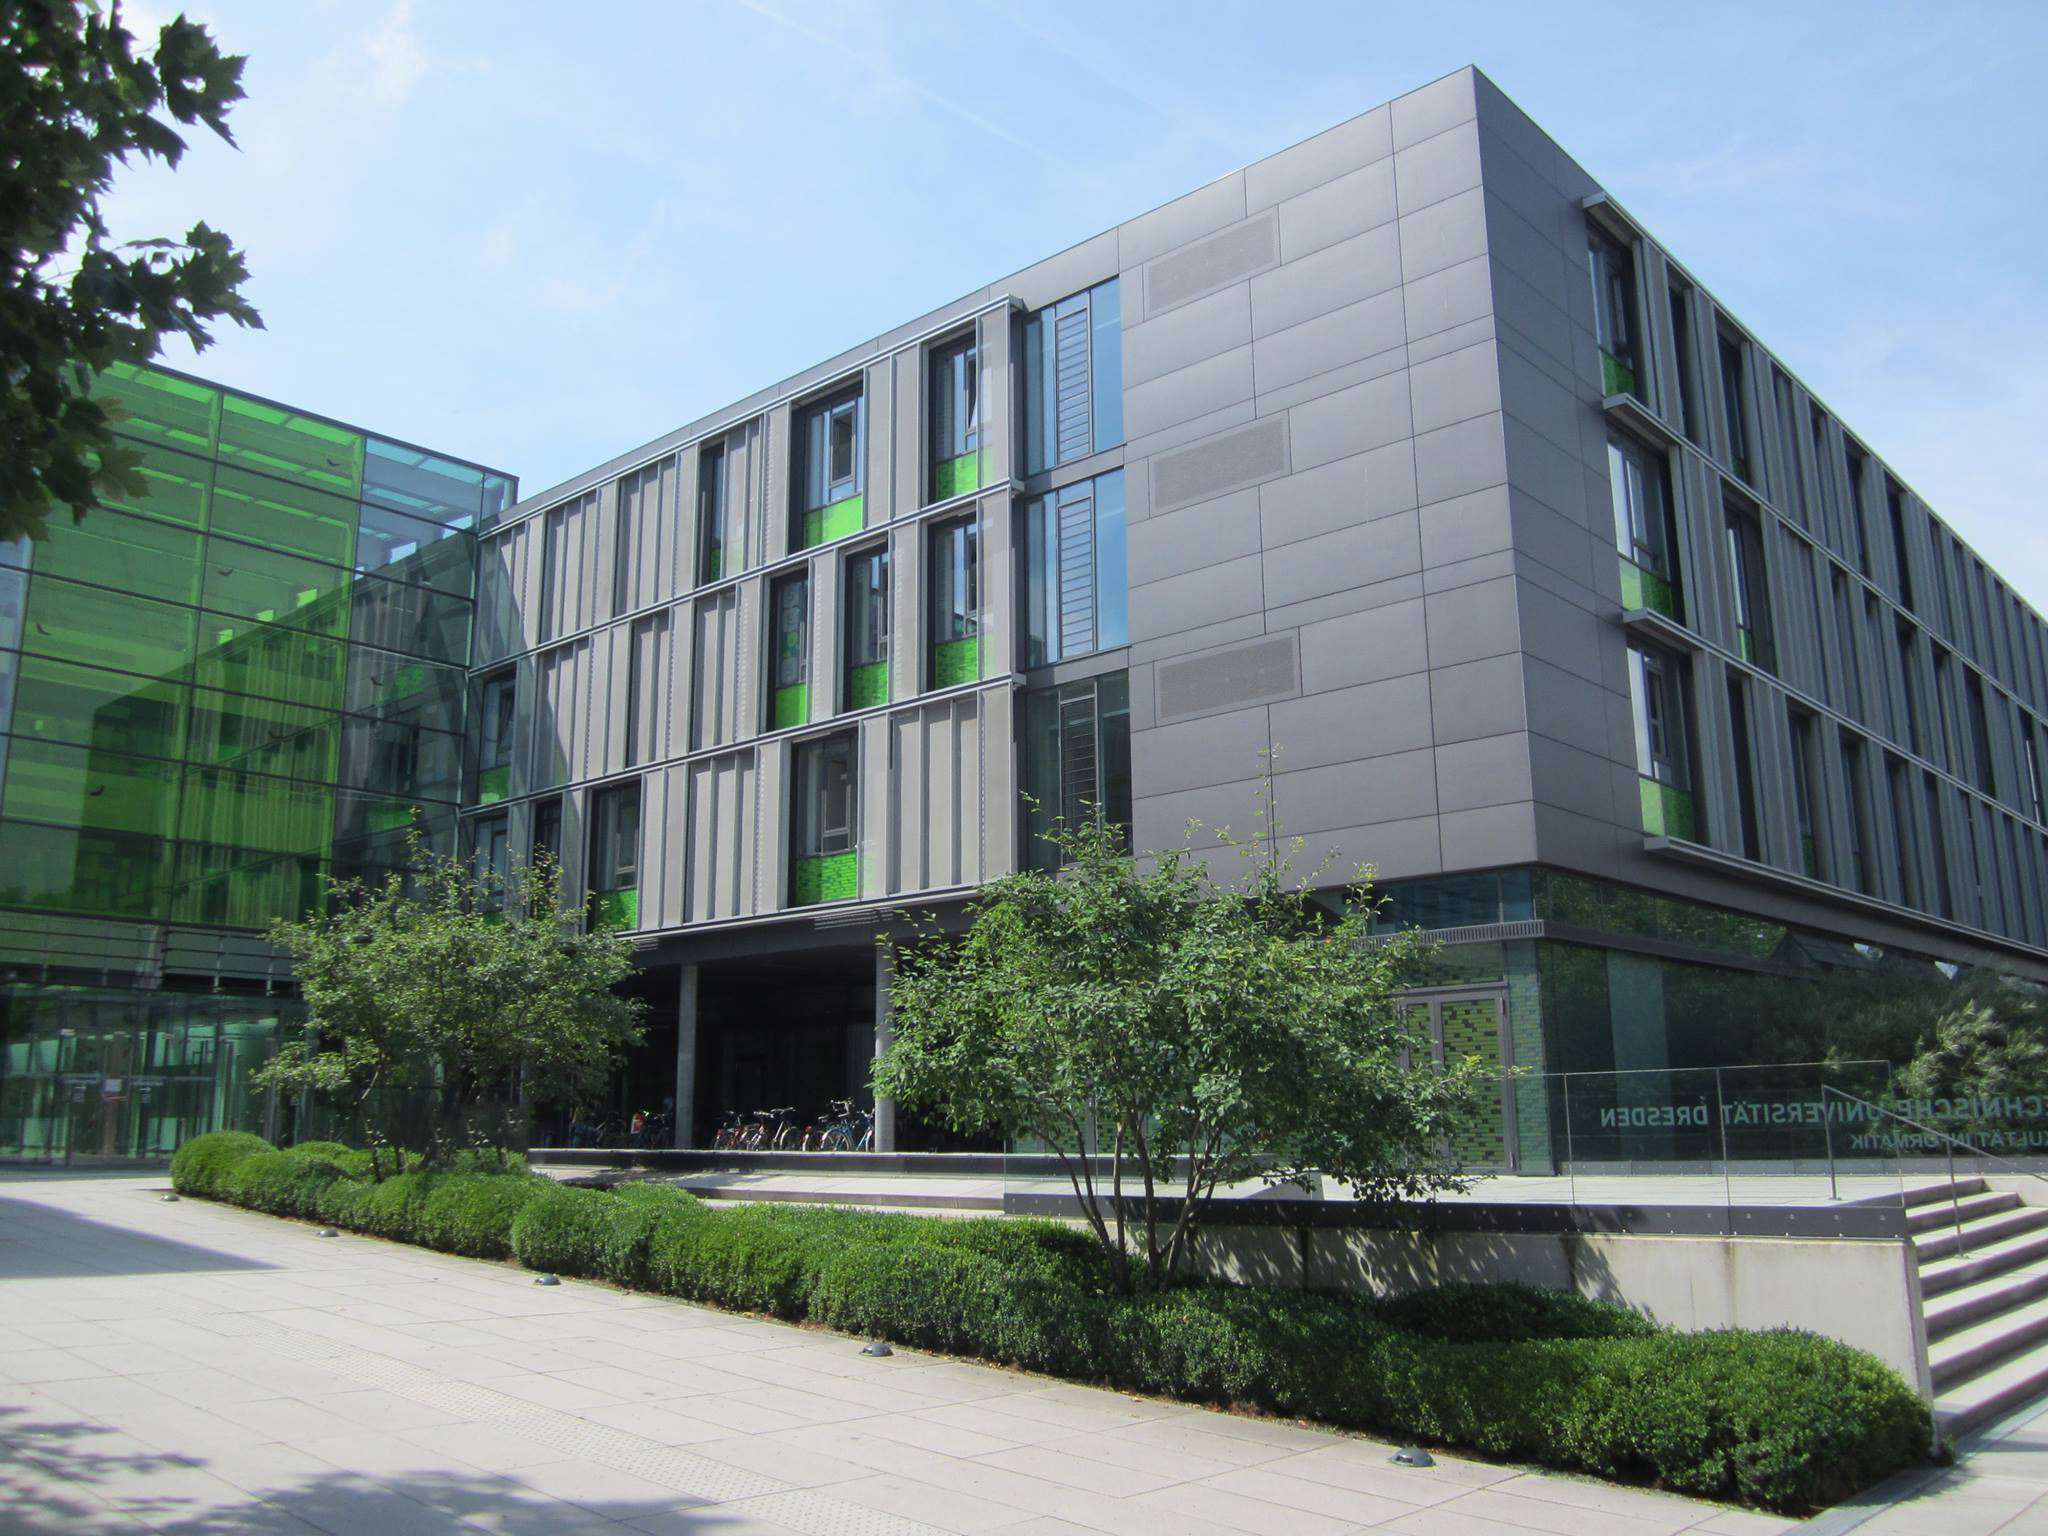
\includegraphics[width=.9\linewidth]{img/fakultaet.jpg}
\caption*{\small \textit{Fakultät Informatik - Foto: Philipp Heisig}}
\end{figure}
